\documentclass[UTF8,twoside,titlepage]{ctexart}

% package
\usepackage{geometry}
\geometry{scale=0.80,a4paper}
\usepackage{multicol}
\usepackage{listings}
\usepackage{graphicx}
\usepackage{float}
\usepackage[format=hang,font=small]{caption}
\usepackage{xcolor}
%for tabular p{} right align
\usepackage{array}
\usepackage{lipsum}
%for long table
\usepackage{longtable}
\usepackage{lscape}

% macro
\newcommand\code[1]{\texttt{#1}}
\newcommand\myref[1]{\ref{#1}(p\pageref{#1})}

\title{OS课设报告 - 任务管理器实现}
\author{王凌峰\thanks{1910630221}}
\date{2021年12月17日}

\begin{document}

%listing setting
\lstset{
    %basicstyle=\small,
    numberstyle=\footnotesize,
    stringstyle=\ttfamily,
    commentstyle=\upshape,
    showstringspaces=false,
    numbers=left,
    numbersep=8pt,
    tabsize=4,
    language=C++
}

\maketitle

\tableofcontents

\section{简介}
% 为何使用C++……
% 实现了哪些功能,没实现哪些……图片……主要分为GUI和windows接口部分,使用的是win32 API和Qt 6.2.2,遵循GPLv3……Qt是庞大C++库,只使用了GUI部分……
% 支持的硬件平台和软件平台……
% 总代码量

\subsection{概览}
此任务管理器使用了Win32 API和Qt的GUI库,语言是C++。仿照Windows 10任务管理器的风格实现了:

\begin{itemize}
    \item 显示所有进程的信息(图标,可执行文件名称,PID,优先级,内存使用,线程数量,所属用户)
    \item 可选择以详细列表或图标形式显示进程信息,以详细列表显示时可以以任何一个属性升序或降序排序
    \item 通过右键菜单结束选中进程
    \item 显示不同用户开启的进程,支持按用户展开和折叠
    \item 创建新进程。可以向新进程传递命令行参数,如果指定的路径不是可执行文件,能根据文件的类型调用合适的应用程序打开
    \item 可以选择3种预设的刷新频率,可以立即刷新
    \item 可通过菜单栏关机或注销
    \item 可使窗口始终在最前
    \item 读取CPU逻辑内核个数,在图表中实时显示60s内各个内核及平均的利用率
    \item 显示CPU的具体型号,基准频率以及所有逻辑内核平均的实时频率
    \item 实时显示系统中进程、线程、句柄总数,以及系统正常运行时间
    \item 显示内存总量和内存利用率,并在图表中实时显示60s内已使用内存的变化情况
    \item 实时显示使用中、可用、已提交、已缓存、分页缓冲池,非分页缓冲池的大小
    \item 帮助菜单栏中有关于本软件和关于Qt的按钮
\end{itemize}

此任务管理器实现的主要是Windows 10任务管理器的``性能''、``用户''和``详细信息''三个页面。GUI风格见图\myref{fig:detailtab}、图\myref{fig:usertab}、图\myref{fig:perftab},菜单栏项目见图\myref{fig:file}、图\myref{fig:option}、图\myref{fig:check.rate}、图\myref{fig:check.view}、图\myref{fig:shut}、图\myref{fig:hlep}、图\myref{fig:about}。

\begin{figure}[htb]
    \centering
    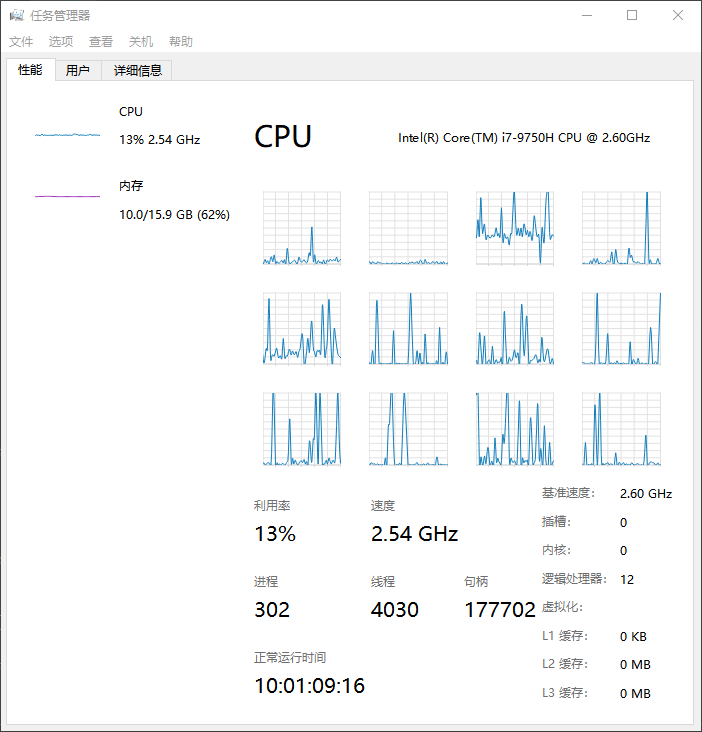
\includegraphics[scale=0.75]{../media/tabs/perfTab/cpu.png}
    \caption{性能页-CPU}
    \label{fig:perftab}
\end{figure}

\begin{figure}[htb]
    \centering
    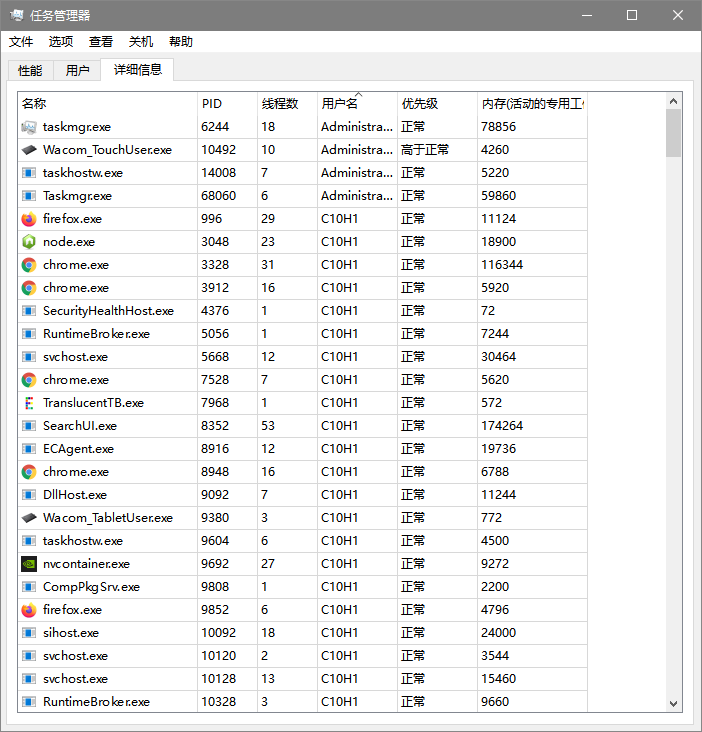
\includegraphics[scale=0.75]{../media/tabs/detailTab/listView/listview.png}
    \caption{详细信息页-详细表格视图(以用户名升序排序)}
    \label{fig:detailtab}
\end{figure}

\begin{figure}[htb]
    \centering
    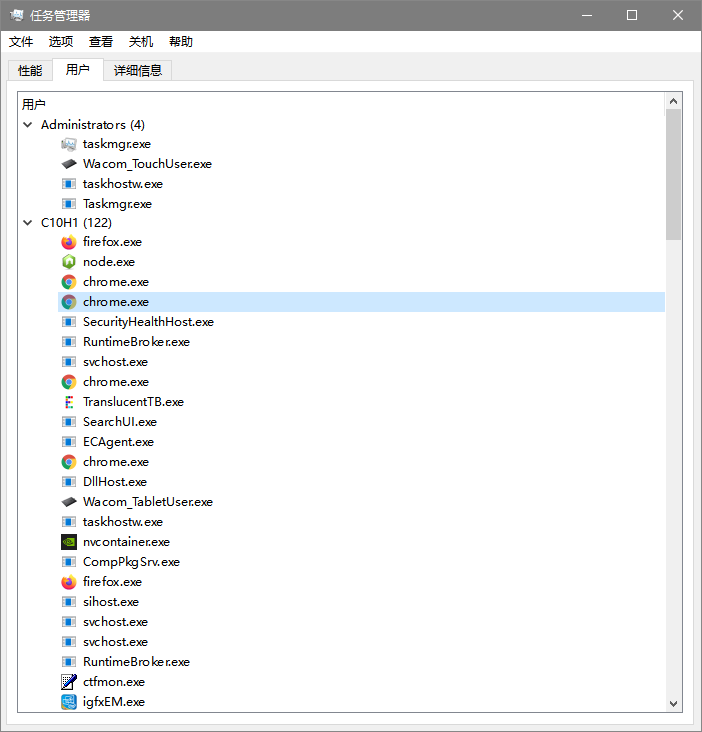
\includegraphics[scale=0.75]{../media/tabs/userTab/usertab expanded.png}
    \caption{用户页(已展开)}
    \label{fig:usertab}
\end{figure}

\begin{figure}[htbp]
    \centering
    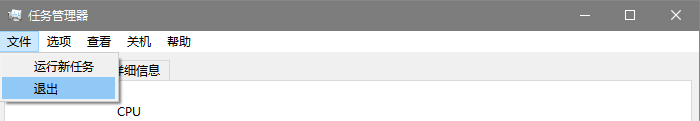
\includegraphics[scale=0.68]{../media/menubar/file menubar.png}
    \caption{文件菜单}
    \label{fig:file}
\end{figure}

\begin{figure}[htbp]
    \centering
    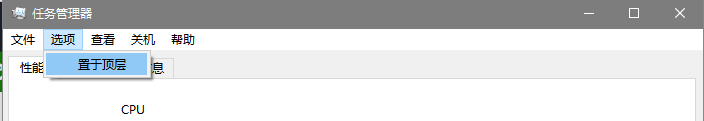
\includegraphics[scale=0.68]{../media/menubar/option menubar.png}
    \caption{选项菜单}
    \label{fig:option}
\end{figure}

\begin{figure}[htbp]
    \centering
    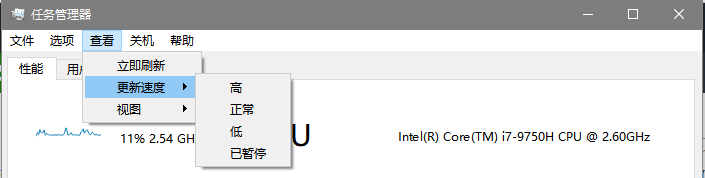
\includegraphics[scale=0.68]{../media/menubar/check menubar rate.png}
    \caption{查看菜单-更新速度}
    \label{fig:check.rate}
\end{figure}

\begin{figure}[htbp]
    \centering
    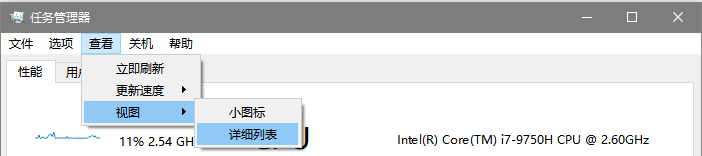
\includegraphics[scale=0.68]{../media/menubar/check menubar view.png}
    \caption{查看菜单-视图}
    \label{fig:check.view}
\end{figure}

\begin{figure}[htbp]
    \centering
    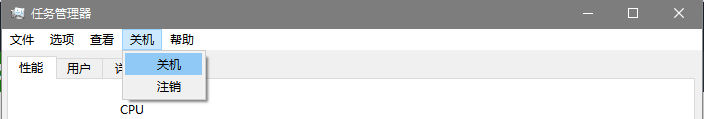
\includegraphics[scale=0.68]{../media/menubar/shutdown menubar.png}
    \caption{关机菜单}
    \label{fig:shut}
\end{figure}

\begin{figure}[htbp]
    \centering
    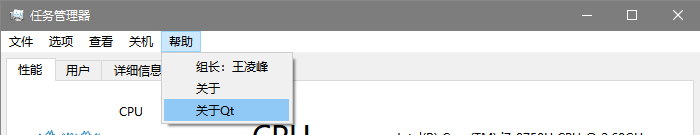
\includegraphics[scale=0.68]{../media/menubar/help menubar.png}
    \caption{帮助菜单}
    \label{fig:hlep}
\end{figure}

\begin{figure}[htb]
    \centering
    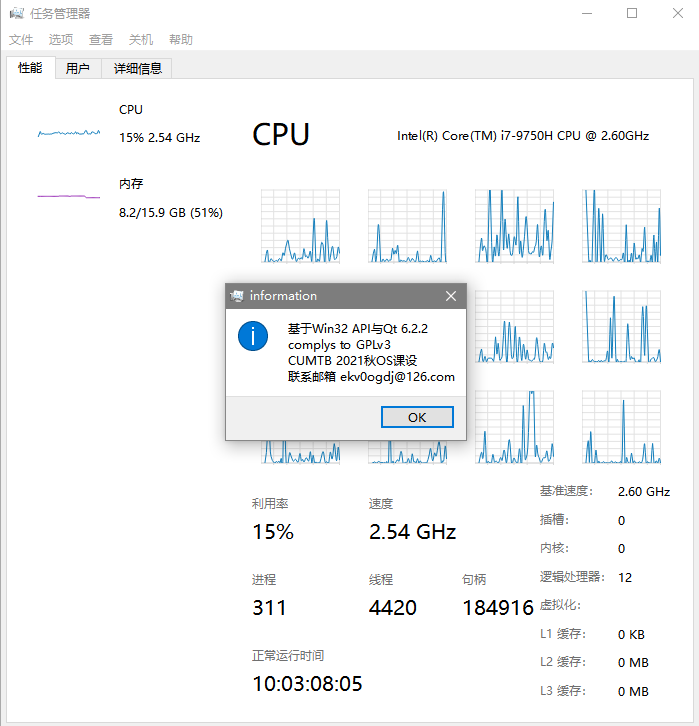
\includegraphics[scale=0.75]{../media/menubar/about dialog.png}
    \caption{关于本项目}
    \label{fig:about}
\end{figure}

没有实现的是应用程序管理和联网状态。由于win10任务管理器没有专门的联网状态信息,而在性能页中显示实时网速成本太高,所以我决定不实现。应用程序管理没有实现的原因是我没观察出win10任务管理器的进程页中判定一个进程属于应用还是后台进程的规则;图形界面程序并不都属于应用,而应用中也不全是图形界面程序。

为了方便,在下文中称此任务管理器为Taskmgr。

\subsection{使用的API与库}
Taskmgr主要分为两部分:GUI部分,调用Windows接口的部分。

调用Windows接口的部分使用的操作系统API是win32 API。win32 API提供了大量关于系统的API,C++是官方推荐的win32 API调用语言之一。

GUI使用Qt的GUI库。Qt是庞大的跨平台C++开发框架,广泛应用于GUI开发。Qt库含有各种模块,其中可能也有对Windows API的包装,但此项目只使用了Qt的GUI库,与GUI无关的部分都由另一个部分完成。

Taskmgr使用遵循GPLv3协议的开源版Qt 6.2.2,因此Taskmgr也遵循GPLv3。(虽然作为课设没什么实际意义)

\subsection{其他}
代码总行数:2354。(不包括Qt Creator自动生成的配置代码)

\section{总体结构}
% 需求就是刚才讲过的功能,当然有几个比较次要的功能还没实现……列出所有要实现的功能
% 主要采用OOP……对象模型(没什么继承关系,简单)……由哪些类组成……不同类的作用……封装性……buffer……win32 API,标准C++类型……
% 功能模型(DFD)……动态模型(事件跟踪图/状态图/SM?)……模块调用(层次方框图?)……
% 模块独立性分析……虽然出现了内容耦合,但程序规模很小且消除这种耦合十分容易。在性能分析一节可以看到性能瓶颈在系统调用上,为了性能是值得的。

\subsection{需求分析}
\label{sec:request}
需求主要就是前文提到的已经实现的功能加上以下还未实现的比较次要的功能:

\begin{itemize}
    \item 显示CPU物理内核数量
    \item 显示CPU L1, L2, L3缓存大小
    \item 显示CPU插槽数
    \item 显示CPU是否支持虚拟化
    \item 显示内存插槽数
    \item 显示内存频率
    \item 显示内存外形规格
    \item 显示为硬件保留的内存
\end{itemize}

\subsection{开发方法与软件结构}
主要采用面对对象的开发方法。

类间没有继承关系,比较简单。具体见表\myref{table:classes}。
\begin{table}[htb]
    \centering
    \begin{tabular}{rl}
        \hline
        类 & 描述 \\
        \hline
        \code{Taskmgr} & 主窗口 \\
        \code{performance} & 性能页 \\
        \code{cpuPage} & 性能页中CPU页面 \\
        \code{memPage} & 性能页中内存页面 \\
        \code{thumbnail} & 性能页中左侧缩略图 \\
        \code{load} & 在性能页中绘制图表的类 \\
        \code{user} & 用户页 \\
        \code{detail} & 详细信息页 \\
        \code{win32\_common} & 调用win32 API的封装类 \\
        \hline
    \end{tabular}
    \caption{任务管理器项目中的类}
    \label{table:classes}
\end{table}

\code{win32\_common}类是对win32 API的封装,提供了各种\code{get}方法获取系统相关信息,还避免了win32 API返回的Windows定义类型(如\code{TCHAR}, \code{DWORD}等)带来的麻烦,因为所有Windows定义类型都限制在类的内部。\code{win32\_common}所有公开函数的传入参数和传出参数都是标准C++类型(如\code{std::string}, \code{std::vector}等)。\code{win32\_common}内所有函数的声明见第\ref{sec:win32api} 节(p\pageref{sec:win32api})。

win32 API中查询函数返回的通常是一个结构体,结构体中包含几种相关的信息。为了不在调用几种请求的数据性质类似的\code{get}函数时重复调用相同的API,\code{win32\_common}内设置了缓冲区。与其他可能被请求的信息存在同一个结构体的数据都存入\code{win32\_common}内的缓冲区,调用相应的\code{get}方法时直接返回缓冲区中的值。缓冲区的刷新通过\code{win32\_common::refresh()}完成。

其余的类都是继承自\code{QWidget}的Qt类,作用是获取、显示系统数据和与用户交互。这些类代表的图形组件之间存在组成关系,例如主窗口由性能页、用户页与详细信息页组成,性能页又由CPU页面、内存页面和略缩图组成,等等。组成关系见本项目的层次方框图(p\pageref{fig:ccfk})。

\begin{figure}
    \centering
    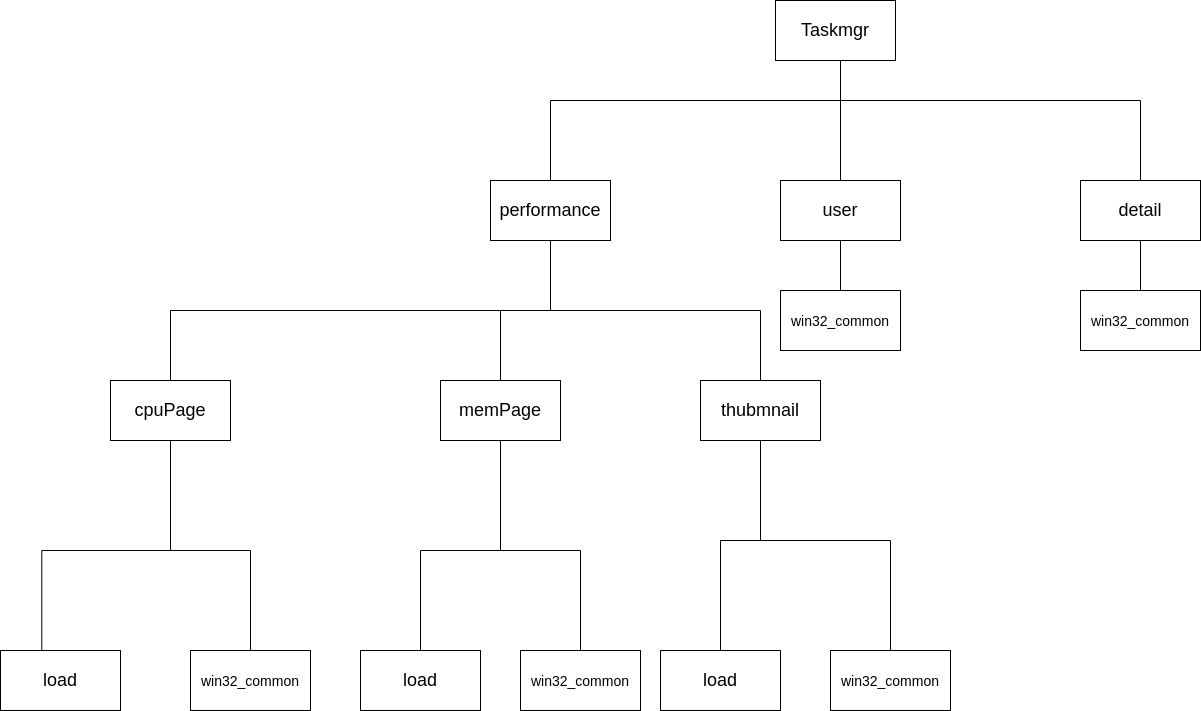
\includegraphics[angle=90,scale=0.5]{../dia/层次方框图.png}
    \caption{层次方框图}
    \label{fig:ccfk}
\end{figure}

Taskmgr中的数据流图非常简单,见图\myref{fig:dfd}。

\begin{figure}[htb]
    \centering
    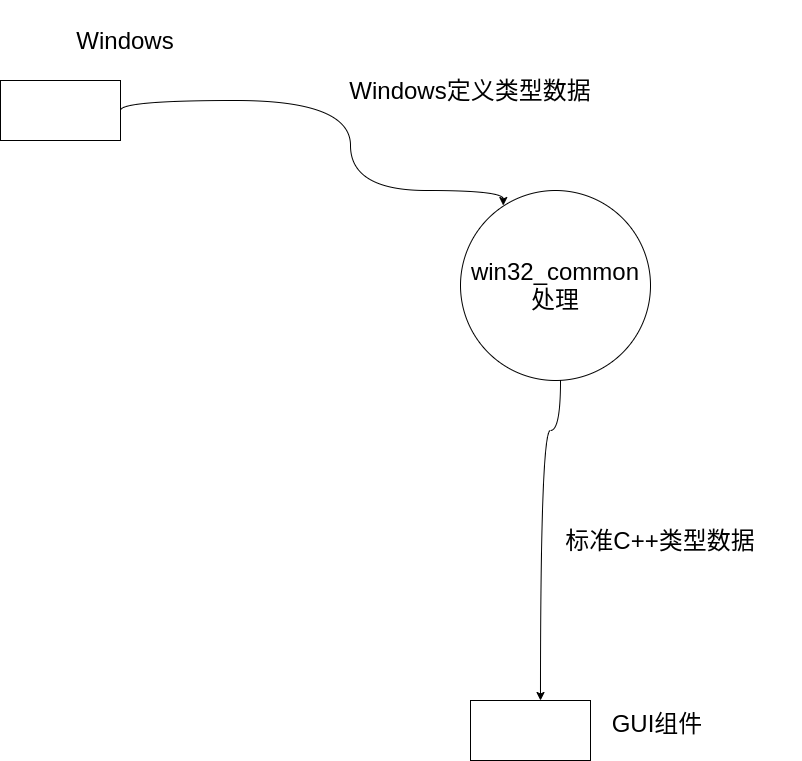
\includegraphics[scale=0.32]{../dia/DFD.png}
    \caption{DFD}
    \label{fig:dfd}
\end{figure}

所有类都有一个\code{refresh()}函数(\code{Taskmgr}类中是\code{do\_refresh()}),用于刷新自身及包含的所有组件。Taskmgr的刷新通过这种递归刷新实现,见图\myref{fig:call}。

\begin{figure}
    \centering
    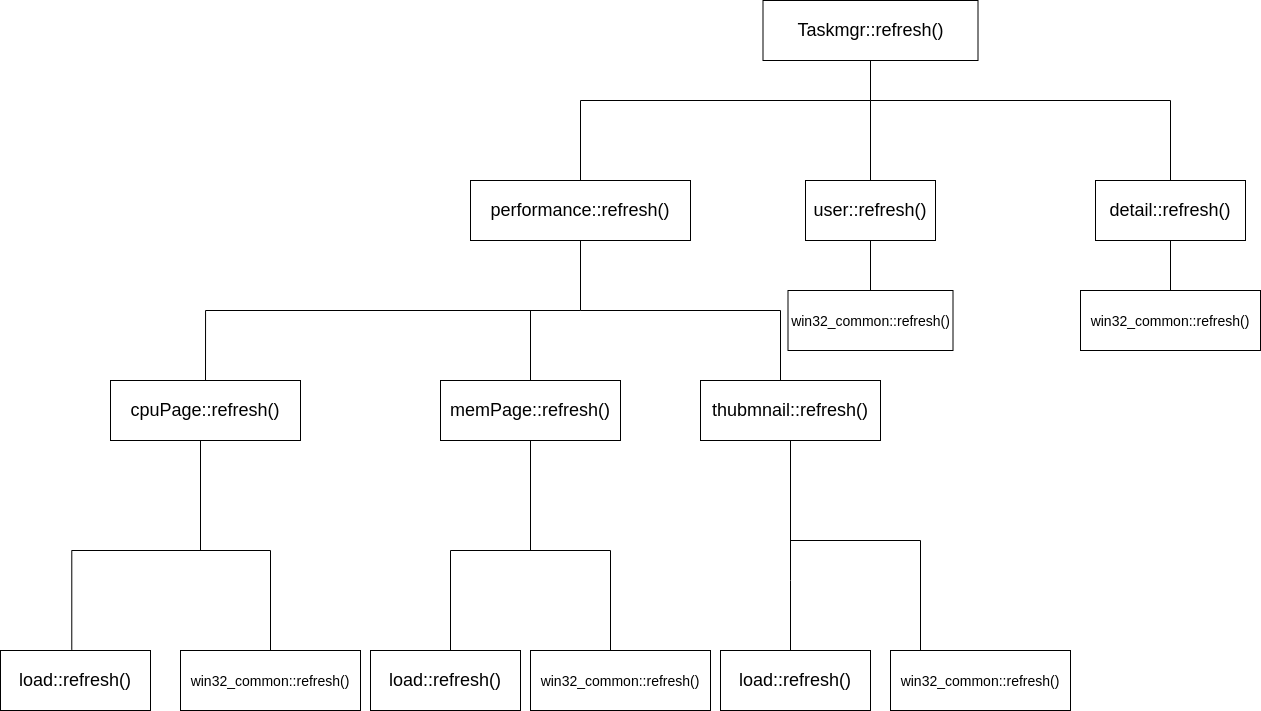
\includegraphics[angle=90,scale=0.5]{../dia/refresh call.png}
    \caption{\code{refresh()}调用关系}
    \label{fig:call}
\end{figure}

\subsection{模块独立性分析}
为了避免每个的需要访问\code{win32\_common}类中非静态类型(具体非静态函数见第\ref{sec:win32api}节(p\pageref{sec:win32api}))的类在被其parent类(Qt中parent与child的概念见第\ref{sec:gui} 节(p\pageref{sec:gui}))调用\code{refresh()}时都刷新一次\code{win32\_common}缓存区,增加不必要的开销,将\code{win32\_common}类移入\code{Taskmgr},其他类只保留指向\code{win32\_common}的指针。刷新时,由\code{Taskmgr}先对\code{win32\_common}进行一次刷新,其余类刷新时只调用\code{get}方法即可。

不过这样就使其他类访问了\code{Taskmgr}类内部的数据,出现了内容耦合。内容耦合应该避免,但在这个项目中我认为是合理的,主要原因有:
\begin{enumerate}
    \item 本项目规模很小,存在一定的高耦合也不是不能接受的
    \item 消除这种耦合十分容易,只要修改有组成关系的Qt类的构造函数和析构函数即可
    \item 如果程序在后续需要增加新功能,很可能仍然使用扩充后的\code{win32\_common}类,这种内容耦合的结构实际上表明了软件的性质,没有必要强行遵循一般的模块独立性准则
    \item 最重要的是这种结构显著提升了程序性能。在第\ref{sec:analyze} 节(p\pageref{sec:analyze})性能分析中,可以看到win32 API调用是Taskmgr的性能瓶颈,应该尽量减少\code{win32\_common::refresh()}调用的次数。
\end{enumerate}

\section{win32 API}
\label{sec:win32api}
% 什么是win32 api,官方文档可查……win32 api使用方法,包含头文件,.pro中指定头文件包含路径和静态链接库路径……
% 本项目封装的功能……
% 本节说明方法,约定的记号……
% 失败的处理……返回值……供调用模块选择

%也许在这里描述接下来的描述方法和记号

\subsection{在程序中使用win32 API的方法}
win32 API以在源代码中\code{\#include}头文件并指定库文件的方式使用。一些Windows上的C++标准库,如MinGW自带一些windows头文件,但由于不是C++标准库,不能保证不缺少文件以及文件的新旧。应该使用Windows SDK中的头文件与库。

Taskmgr项目使用qt creator作为IDE,项目管理文件是一个\ .pro文件。为了使用win32 API,需要在\ .pro文件中指明头文件路径与需要使用的库:

\begin{quote}
\ttfamily
win32: LIBS += -lPdh \
                -lpowrprof

INCLUDEPATH += 'D:/Program Files (x86)/Windows Kits/10/Include/10.0.22000.0'

DEPENDPATH += 'D:/Program Files (x86)/Windows Kits/10/Include/10.0.22000.0'
\end{quote}

\subsection{\code{win32\_common}封装的功能}
\code{win32\_common}要提供的在系统运行中可能实时变化的Windows的属性以及这些属性所属的结构体见表\myref{table:field.struc}。找出所有含有一个以上\code{win32\_common}需要提供的动态变化的属性的结构体,这些结构体中\code{win32\_common}需要的属性可能在一个刷新周期内被\code{win32\_common}访问不止一个,所以需要全部放进缓存区。由于与\code{win32\_common}实例的状态有关,缓存区中属性对应的\code{get}函数自然是非静态的,而其他的都是静态函数。

\begin{table}[htb]
    \centering
    \begin{tabular}{rl}
        \hline
        含义 & Windows结构体中的属性 \\
        \hline
        PID & \code{PROCESSENTRY32.th32ProcessID} \\
        进程的线程数 & \code{PROCESSENTRY32.cntThreads} \\
        进程映像文件名称 & (无,直接由\code{GetModuleBaseName()}获得) \\
        进程映像文件路径 & (无,直接由\code{GetModuleFileNameEx()}获得) \\
        进程优先级 & (无,直接由\code{GetPriorityClass()}获得) \\
        进程占有的物理内存 & \code{PROCESS\_MEMORY\_COUNTERS.WorkingSetSize} \\
        进程所属的用户名 & (无,由\code{LookupAccountSid()}获得) \\
        CPU时钟频率(MHz) & \code{PROCESSOR\_POWER\_INFORMATION.CurrentMhz} \\
        CPU利用率 & \code{PDH\_FMT\_COUNTERVALUE} \\
        系统中进程数 & \code{PERFORMACE\_INFORMATION.ProcessCount} \\
        系统中线程数 & \code{PERFORMACE\_INFORMATION.ThreadCount} \\
        系统中句柄数 & \code{PERFORMACE\_INFORMATION.HandleCount} \\
        系统启动以来的时间(ms) & (无,直接由\code{GetTickCount()}获得) \\
        物理内存大小(B) & \code{PERFORMACE\_INFORMATION.PhysicalTotal} \\
        可用物理内存(B) & \code{PERFORMACE\_INFORMATION.PhysicalAvailable} \\
        已提交内存(B) & \code{PERFORMACE\_INFORMATION.CommitTotal} \\
        系统已缓存内存(B) & \code{PERFORMACE\_INFORMATION.SystemCache} \\
        分页缓冲池(B) & \code{PERFORMACE\_INFORMATION.KernelPaged} \\
        非分页缓冲池(B) & \code{PERFORMACE\_INFORMATION.KernelNonpaged} \\
        \hline
    \end{tabular}
    \caption{\code{win32\_common}提供的可能实时变化的信息及其所在的结构体}
    \label{table:field.struc}
\end{table}

全部的函数声明见下表:

{
    \ttfamily
    \centering
    \begin{longtable}{>{\raggedleft\arraybackslash}p{18em}p{24em}}
        \hline
        bool & refresh() \\
        const std::map<unsigned long,unsigned long long>\& & getPid\_Thrdcnt() const \\
        static bool & getProcName(unsigned long pid,std::string \&name) \\
        static bool & getProcPath(unsigned long pid,std::string \&path) \\
        static bool & getProcCla(unsigned long pid,std::string \&cla) \\
        static bool & getProcMem(unsigned long pid,unsigned long long \&mem) \\
        static bool & getProcUserName(unsigned long pid,std::string \&username) \\
        static bool & killProc(const unsigned long pid) \\
        unsigned & getLogicCpuCnt() const \\
        double & getCpuLoad(unsigned n) const \\
        unsigned long long & getProcCnt() const \\
        unsigned long long & getThrdCnt() const \\
        unsigned long long & getHandlCnt() const \\
        std::string & getCpuInfo() const \\
        double & getCpuClock() const \\
        double & getCpuBaseClock() const \\
        static std::string & getTimeSinceStart() \\
        unsigned & getCpuSlot() const \\
        unsigned & getCpuCoreCnt() const \\
        std::string & getVl() const \\
        unsigned long & getL1Cache() const \\
        unsigned long & getL2Cache() const \\
        unsigned long & getL3Cache() const \\
        unsigned long & getMemLoad() const \\
        double & getPhyTot() const \\
        double & getPhyAvail() const \\
        double & getPhyUsed() const \\
        double & getCommTot() const \\
        double & getSysCache() const \\
        double & getPaged() const \\
        double & getNonpaged() const \\
        unsigned long & getMemSpeed() const \\
        unsigned & getMemUsedSlot() const \\
        unsigned & getMemTotSlot() const \\
        std::string & getMemShape() const \\
        unsigned long & getMemReserved() const \\
        static std::string & to\_str(TCHAR *tc) \\
        static bool & openProc(const char *path,const char *params,bool asAdmin) \\
        static bool & shutdown() \\
        static bool & logoff() \\
        static bool & getShutdownPriv() \\
        unsigned long long & getPageSz() \\
        \hline
    \caption{\code{win32\_common}的函数声明}
    \label{table:win32func}
    \end{longtable}
}

很多\code{get}函数的返回值是\code{bool},指示是否运行成功。另外,所有函数中在获取要求的属性前将输出变量设置为能够指示成功与否的值。例如在\code{getProcName()}中:

{
    \ttfamily
    \lstinputlisting[breaklines=true,linerange={60-62},firstnumber=60]{../source/win32_common.cc}
}

在Taskmgr中,使用后一种方式,函数运行失败后使用\code{"unknown"}, \code{0}这类明显错误的值。

\subsection{\code{win32\_common}的实现}

接下来描述\code{win32\_common}中一些函数的实现思路。

\subsubsection{\code{pid\_thrd}的获取}
\code{pid\_thrd}是\code{win32\_common}内部的\code{map}容器,包含所有进程PID到其线程数的映射。

首先向\code{CreateToolhelp32Snapshot()}的\code{dwFlags}参数传递\code{TH32CS\_SNAPPROCESS}获得系统中所有进程的快照\footnote{https://docs.microsoft.com/en-us/windows/win32/api/tlhelp32/nf-tlhelp32-createtoolhelp32snapshot},再用\code{Process32First()}和\code{Process32Next()}取出系统快照中每个进程的信息,依次存入\code{PROCESSENTRY32}结构\footnote{https://docs.microsoft.com/en-us/windows/win32/api/tlhelp32/nf-tlhelp32-process32first}。主要代码见图\myref{code:pidthrd}。

\begin{figure}[H]
    \ttfamily
    \lstinputlisting[breaklines=true,linerange={303-316},firstnumber=303]{../source/win32_common.cc}
    \caption{\code{win32\_common.cc::refresh()}}
    \label{code:pidthrd}
\end{figure}

一个\code{PROCESSENTRY32}结构包含一个进程的相关信息,其中的\code{th32ProcessID}和\code{cntThreads}字段分别是该进程的PID和线程数\footnote{https://docs.microsoft.com/en-us/windows/win32/api/tlhelp32/ns-tlhelp32-processentry32},在\code{win32\_common::refresh()}中将映射关系存入\code{map}容器即可。

不分别获取PID和对应的线程数是因为Windows似乎没有提供通过PID获取线程数的API,如果不通过\code{PROCESSENTRY32}或\code{THREADENTRY32}\footnote{https://docs.microsoft.com/en-us/windows/win32/api/tlhelp32/ns-tlhelp32-threadentry32}预先保存系统快照中的(PID,线程数)对,就需要在获取线程数时遍历线程的快照,计算创建它的进程的PID与请求的PID相同的数量,复杂度为$O(N^2)$。

\subsubsection{进程名的获取}
Windows中,Module是一个可执行文件或DLL,每个进程都由一个或多个module组成\footnote{https://docs.microsoft.com/en-us/windows/win32/psapi/module-information},进程的名称就是该启动该进程的可执行文件或DLL文件的文件名。



\code{GetModuleBaseName()}接收一个进程句柄和一个模块句柄,返回该模块的模块名\footnote{https://docs.microsoft.com/en-us/windows/win32/api/psapi/nf-psapi-getmodulebasenamew}。模块句柄的获得通过\code{EnumProcessModules},设置\code{cb}参数为一个模块句柄的大小以获得一个模块句柄\footnote{https://docs.microsoft.com/en-us/windows/win32/api/psapi/nf-psapi-enumprocessmodules}。

\code{OpenProcess()}根据PID返回对应进程的句柄。值得注意的是需要在\code{OpenProcess()}的\code{dwDesiredAccess}参数中指定对进程对象的访问权限\footnote{https://docs.microsoft.com/en-us/windows/win32/api/processthreadsapi/nf-processthreadsapi-openprocess}。为了获取进程的模块,需要\code{PROCESS\_QUERY\_INFORMATION}和\code{PROCESS\_VM\_READ}权限\footnote{https://docs.microsoft.com/en-us/windows/win32/procthread/process-security-and-access-rights}。

代码如下:

\begin{figure}[H]
    \ttfamily
    \lstinputlisting[breaklines=true,linerange={60-80},firstnumber=60]{../source/win32_common.cc}
    \caption{\code{win32\_common::getProcName()}}
\end{figure}

\subsubsection{module路径的获取}
这个功能在获取进程的图标时使用。

类似于\code{GetModuleBaseName},\code{GetModuleFileNameEx}返回进程的模块的完整路径\footnote{https://docs.microsoft.com/en-us/windows/win32/api/psapi/nf-psapi-getmodulefilenameexw}。

\subsubsection{进程所属用户的用户名的获取}
Windows中用SID (security identifier)标识用户(user)、组(group)及计算机账户(computer accounts)\footnote{https://docs.microsoft.com/en-us/windows/win32/secgloss/s-gly},为了获取进程所属的用户的名称,要先获取进程所属用户的SID,然后通过\code{LookupAccountSid()}得到SID对应的用户名\footnote{https://docs.microsoft.com/en-us/windows/win32/api/winbase/nf-winbase-lookupaccountsida}。

进程所属用户的SID的获取通过向\code{GetTokenInformation()}的\code{TokenInformationClass}参数传递\code{TokenOwner}得到\footnote{https://docs.microsoft.com/en-us/windows/win32/api/securitybaseapi/nf-securitybaseapi-gettokeninformation}。这个API接收一个access token的句柄为参数,特定进程access token handle的获取通过\code{OpenProcessToken()}\footnote{https://docs.microsoft.com/en-us/windows/win32/api/processthreadsapi/nf-processthreadsapi-openprocesstoken},而该API接收的\code{ProcessHandle}参数由前面介绍的\code{OpenProcess()}得到,其中\code{dwDesiredAccess}为\code{PROCESS\_QUERY\_INFORMATION}。

代码如下:

\begin{figure}[H]
    \ttfamily
    \lstinputlisting[breaklines=true,linerange={157-187},firstnumber=157]{../source/win32_common.cc}
    \caption{\code{win32\_common::getProcUserName()}}
\end{figure}

\subsubsection{结束进程}
结束进程API为\code{TerminateProcess()},获得进程句柄时需要向\code{OpenProcess()}的\code{dwDesiredAccess}参数传递\code{PROCESS\_TERMINATE}\footnote{https://docs.microsoft.com/en-us/windows/win32/api/processthreadsapi/nf-processthreadsapi-terminateprocess}。

代码如下:

\begin{figure}[H]
    \ttfamily
    \lstinputlisting[breaklines=true,linerange={189-200},firstnumber=189]{../source/win32_common.cc}
    \caption{\code{win32\_common::killProc()}}
\end{figure}

\subsubsection{CPU型号的获取}
\code{\_\_cpuid()}产生x86和x64上可用的CPU指令,查询CPU支持的特性和CPU的类型\footnote{https://docs.microsoft.com/en-us/cpp/intrinsics/cpuid-cpuidex?view=msvc-170}。\code{\_\_cpuid()}接收\code{function\_id}参数指定要查询信息的类型。当其为\code{0x80000002},\code{0x80000003},\code{0x80000004}时,分别表示CPU制造商(manufacturer),型号(model),基准频率(Clockspeed)。

代码如下:

{
    \ttfamily
    \lstinputlisting[breaklines=true,linerange={249-269},firstnumber=249]{../source/win32_common.cc}
}

\subsubsection{创建新进程}
\code{ShellExecuteA()}能对文件做一些操作,操作的具体类型由参数\code{lpOperation}指定。\code{lpOperation}可以为\code{edit},\code{open},\code{runas}等,例如对文档类型(document)可以使用\code{edit}打开相应的编辑器,对可执行文件可使用\code{open}执行文件\footnote{https://docs.microsoft.com/en-us/windows/win32/api/shellapi/nf-shellapi-shellexecutea}。

当\code{lpOperation}为\code{NULL}时,系统自动判断\code{lpFile}指向路径的文件或文件夹的类型,并执行该可执行文件或用合适的应用打开文档。这和Win10任务管理器中``运行新任务''菜单栏的功能十分类似。因此Taskmgr中创建新进程使用的API就是\code{ShellExecuteA()}。

\begin{figure}[H]
    \centering
    \ttfamily
    \lstinputlisting[breaklines=true,linerange={4-17},firstnumber=4]{../source/win32_common.cc}
    \caption{\code{win32\_common::openProc()}}
\end{figure}

其中\code{verb}设置为\code{"runas"}时,表示以管理员权限打开应用程序\footnote{https://docs.microsoft.com/en-us/windows/win32/api/shellapi/nf-shellapi-shellexecutea}。这在\ref{elevatepriv} 小节(p\pageref{elevatepriv})Taskmgr提升权限时会用到。

Taskmgr的创建新进程实现了启动可执行文件的同时传递参数的功能。Qt弹出``运行新任务''窗口后调用\code{Taskmgr::parsePath()}分析接受到的字符串(具体见节\myref{sec:gui}),从用户输入中分辨出文件路径和传递的参数,分别存于\code{std::string \&prog}与\code{std::string \&param}中。Taskmgr再将这两个字符串转换为C字符串并作为参数传递给\code{win32\_common::openProc()}函数,即可在Taskmgr中以特定命令行参数启动新进程。

\subsection{Taskmgr的权限提升}
\label{elevatepriv}
%windows权限规则介绍……main.cc如何与win32_common配合……
为了获得足够的权限访问某些进程数据及结束某些进程,Taskmgr需要获得管理员权限。Windows在用户登陆时生成access token,access token 包含该用户及其用户组的权限(privileges),以该用户身份执行的所有进程都包含access token的一个副本。Windows通过access token验证进程执行的操作\footnote{https://docs.microsoft.com/en-us/windows/win32/secauthz/access-control-components}。

所以为了执行必要的操作,access token中需要包括对应的privilege。但access token中的privilege只能使能/激活(enable)已存在的权限\footnote{https://docs.microsoft.com/en-us/windows/win32/secbp/changing-privileges-in-a-token?redirectedfrom=MSDN},也就是说进程的权限只可能在创建前指定。

有几种以管理员权限运行程序的方法,例如右键以管理员身份运行,在manifest文件中指定execution level\footnote{http://msdn.microsoft.com/en-us/library/bb756929.aspx},或者使用Windows自带的\code{runas}命令让普通用户以管理员身份执行程序和命令。

为了方便,Taskmgr在启动时调用\code{win32\_common::openProc()},以管理员身份启动\code{Taskmgr.exe}的另一个副本后结束原进程。\code{win32\_common::openProc()}中根据传递的参数设置verb为\code{"runas"},并将\code{"noadmin"}作为参数传递给新进程(即Taskmgr.exe的副本),新进程接收到此参数后跳过\code{win32\_\linebreak common::openProc()}代码段,进入正常运行。这个行为是在\code{main.cc}中实现的:

{
    \ttfamily
    \lstinputlisting[breaklines=true,linerange={9-19},firstnumber=9]{../source/main.cc}
}

\section{GUI}
\label{sec:gui}
% 界面分解,有哪些部分……Qt中QWidget类的地位,与QMainWindow的关系,parent与child,QWidget组件可加入任何组件……Qt的三种基本布局,本项目的布局……
% 各个部分继承/使用的类,为了达到需要的功能覆盖的超类函数……
% 每个类的DFD/状态图……?
% chart QT += charts……
% Qt中类的destructor写法……
\subsection{界面分解}
Qt中有四种基本的布局:

\begin{itemize}
    \item \code{QVBoxLayout},垂直布局
    \item \code{QHBoxLayout},水平布局
    \item \code{QGridLayout},网格布局
    \item \code{QFormLayout},表单布局
\end{itemize}

为了仿照Win10任务管理器的界面,根据Qt中的布局对Win10任务管理器进行一些分解。见图\myref{fig:layout}。

\begin{figure}[htb]
    \centering
    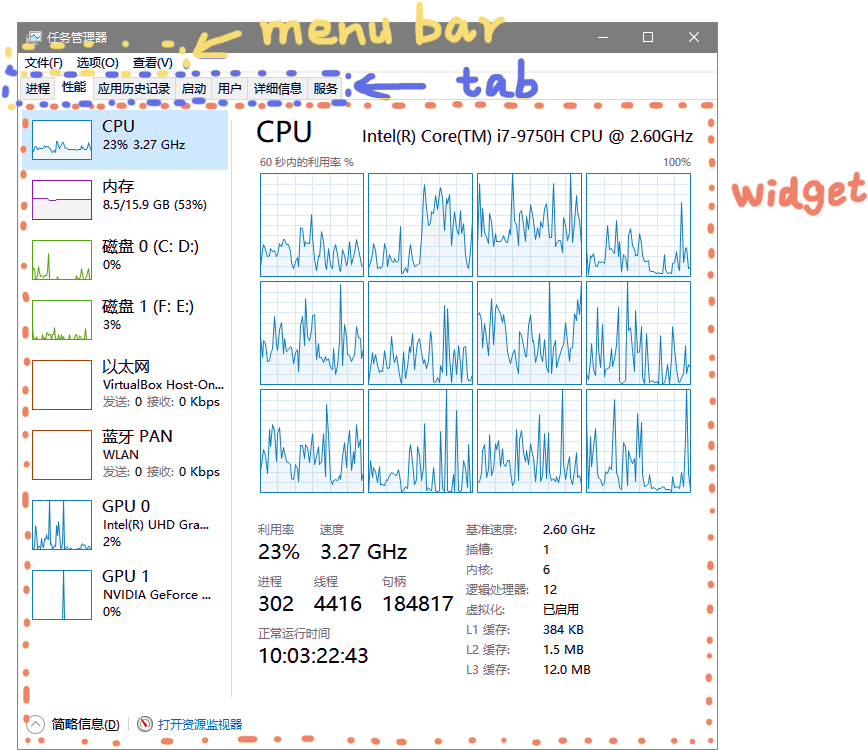
\includegraphics[scale=0.5]{../media/layout/总体布局_2.png}
    \caption{Win10任务管理器的总体布局}
    \label{fig:layout}
\end{figure}

性能页、用户页和详细信息页的切换可以使用\code{QTableWidget}实现,当用户点击不同的Tab,即切换到相应的页面。

Qt中\code{QWidget}可以作为其他\code{QWidget}的parent或child。通过继承\code{QWidget}类,Taskmgr项目中定义的类可以加入其他窗口类中。指定合适的布局,就能得到与Win10任务管理器类似的风格。

具体分解方法和使用的布局以CPU页面为例,见图\myref{fig:cpupage}和图\myref{fig:cpuright}。

\begin{figure}[htb]
    \centering
    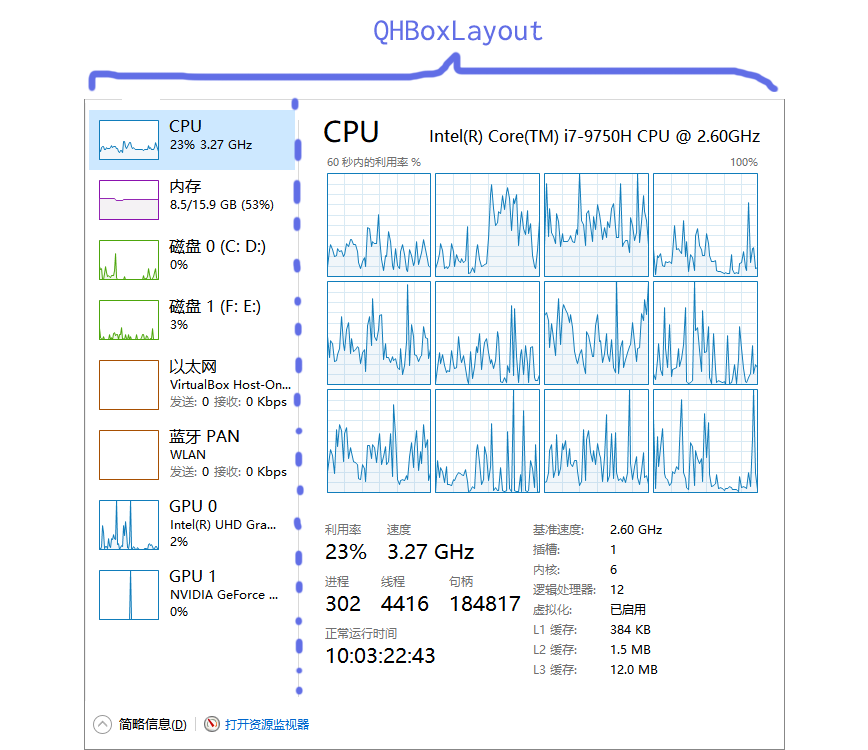
\includegraphics[scale=0.34]{../media/layout/cpupage.png}
    \caption{CPU页面布局}
    \label{fig:cpupage}
\end{figure}

\begin{figure}[htb]
    \centering
    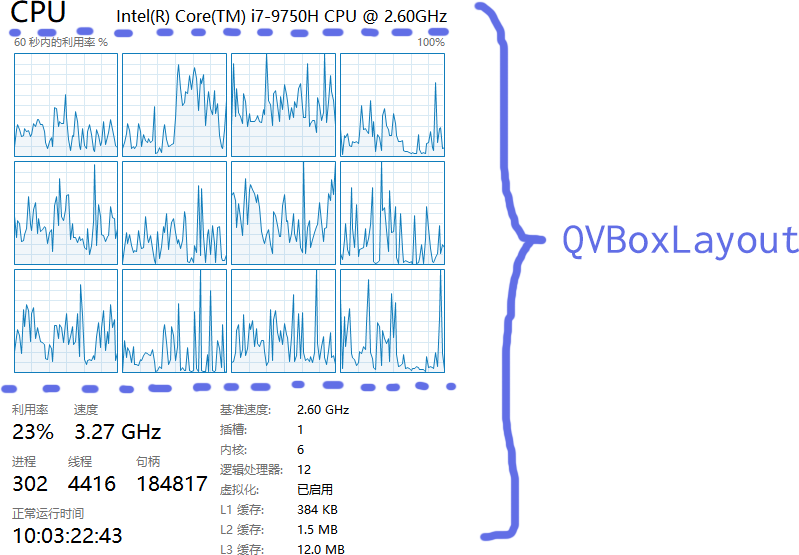
\includegraphics[scale=0.4]{../media/layout/cpupage right.png}
    \caption{CPU页面右侧布局}
    \label{fig:cpuright}
\end{figure}

\subsection{signal与slot}
Qt中signal与slot是不同对象间沟通的机制\footnote{https://doc.qt.io/qt-5/signalsandslots.html},特定操作会发射signal,而与这个signal关联的slot响应signal。

Qt中signal与slot的关联是完成特定功能的重要方式。Taskmgr GUI界面的显示逻辑,与用户的交互,调用\code{win32\_common}类的时机都是通过signal与slot实现的。

大多数Qt组件都预先定义了不少signal,只需要自定义slot并将signal与slot关联即可。不过\code{performance}类中也创建了新的signal\code{clicked},当鼠标点击\code{performance}类时发射此signal,完成一些功能。具体见小节\myref{subsec:perf}。

\subsection{\code{Taskmgr}类的实现}
状态图见图\myref{fig:taskmgrstat}。

\begin{figure}[htb]
    \centering
    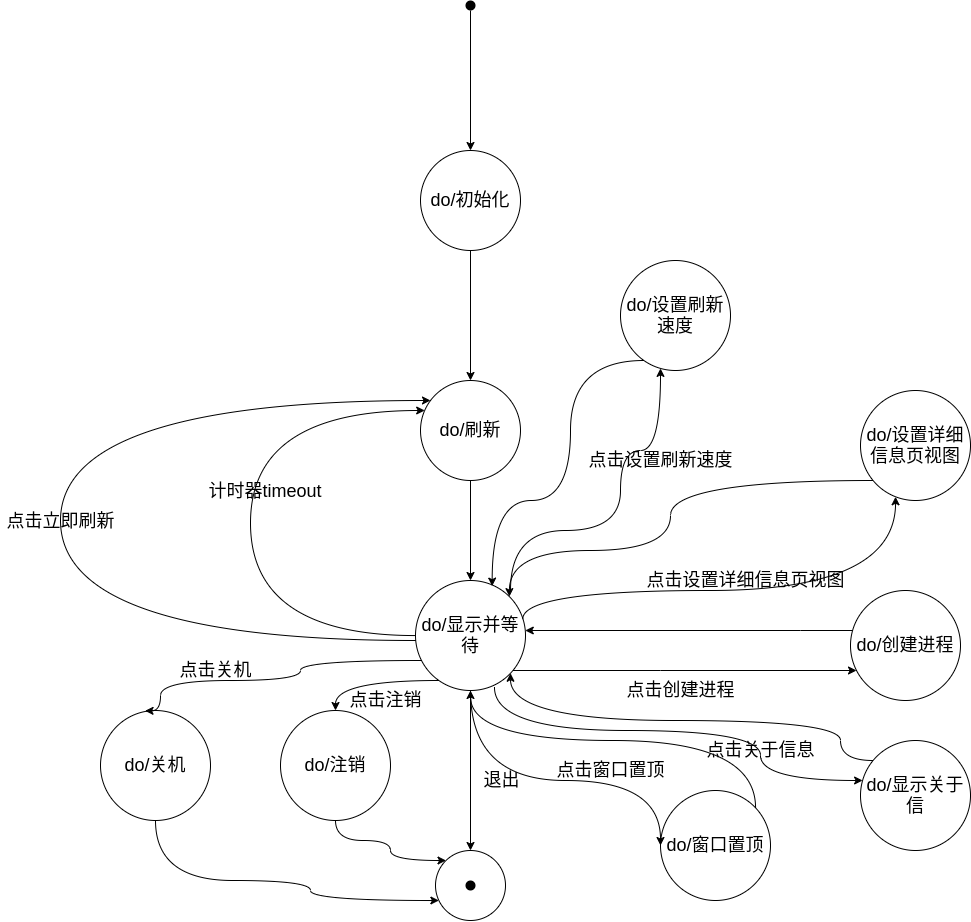
\includegraphics[scale=0.43]{../dia/taskmgr.png}
    \caption{\code{Taskmgr}类状态图}
    \label{fig:taskmgrstat}
\end{figure}

性能页、用户页和详细信息页的切换使用\code{QTableWidget},点击Tab即可切换到相应页面。

定时刷新使用\code{QTimer}类。将signal \code{QTimer::timeout()}与slot \code{Taskmgr::do\_refresh()}关联。使用\code{QAction::setChecked()}确保更新速度默认为正常(1000 ms)。

菜单栏通过创建一个从属于主窗口的\code{QMenuBar}类添加,各个菜单项,如``文件''等,由\code{QMenuBar::\linebreak addMenu()}函数添加。具体的项目,如``退出''等,由\code{QMenu::addAction()}添加。

\code{QAction}类提供了抽象的用户界面的动作,\code{QAction}类的实例可以插入不同的\code{QWidget}组件,并根据所在的组件以不同的风格显示\footnote{https://doc.qt.io/qt-5/qaction.html}。\code{QAction}类有预定义signal \code{QAction::triggered},在\code{QAction}形成的组件被激活时发射。

一组action可以是互斥的,即同一时间只能有一个action被激活。在Taskmgr菜单栏的更新速度菜单中的项目和视图菜单中的项目就属于这种情况。创建一个\code{QActionGoup}实例并把同组动作加入其中即可。

\code{Taskmgr}类中action与slot的对应关系见图\myref{table:actionslot}。

\begin{table}
    \centering
    \ttfamily
    \begin{tabular}{ccc}
        \hline
        action & slot & \normalfont{描述}\\
        \hline
        newProcAc & do\_newProc() & \normalfont{创建新进程}\\
        exitAc & do\_Exit() & \normalfont{退出Taskmgr}\\
        onTopAc & do\_onTop() & \normalfont{窗口始终在最前}\\
        refreshAc & do\_refresh() & \normalfont{立即刷新}\\
        highRateAc & do\_highRate() & \normalfont{高刷新速度}\\
        normRateAc & do\_normRate() & \normalfont{正常刷新速度}\\
        lowRateAc & do\_lowRate() & \normalfont{低刷新速度}\\
        pauseRefreshAc & do\_pauseRefresh() & \normalfont{暂停刷新}\\
        iconViewAc & do\_iconView() & \normalfont{详细信息页图标视图}\\
        listViewAc & do\_listView() & \normalfont{详细信息页详细列表视图}\\
        shutAc & do\_shutdown() & \normalfont{关机}\\
        logOffAc & do\_logOff() & \normalfont{注销}\\
        infoAc & do\_info() & \normalfont{关于信息}\\
        qtInfoAc & do\_qtInfo() & \normalfont{关于Qt}\\
        nameAc & do\_info() & \normalfont{关于信息}\\
        \hline
    \end{tabular}
    \caption{\code{Taskmgr}类中action与相应的处理函数}
    \label{table:actionslot}
\end{table}

在\code{do\_newProc()}中,首先使用\code{QInputDialog::getText()}函数弹出窗口提示用户输入路径,规则是:可以输入可执行文件路径,也可输入其他类型文件或文件夹路径;可以向可执行文件传递参数;路径中若出现空格,需要使用双引号包围。

收到用户输入后调用\code{Taskmgr::parsePath()}得到文件路径和命令行参数的字符串,再根据这两个信息调用\code{win32\_common::openProc()}打开新进程。

\code{Taskmgr::parsePath()}代码如下:

{
    \ttfamily
    \lstinputlisting[breaklines=true,linerange={259-297},firstnumber=259]{../source/taskmgr.cc}
}

\subsection{详细信息页的实现}
状态图见图\myref{fig:detailstat}。

\begin{figure}[htb]
    \centering
    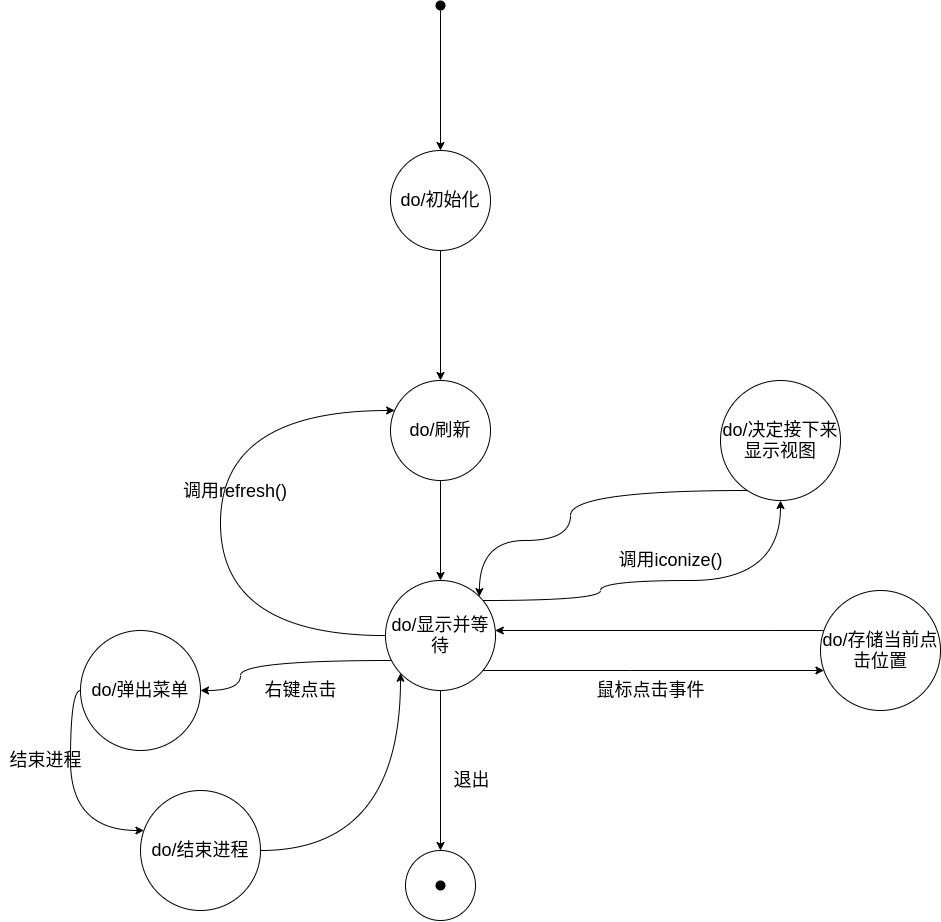
\includegraphics[scale=0.42]{../dia/detail.png}
    \caption{\code{detail}类状态图}
    \label{fig:detailstat}
\end{figure}

详细信息页有两种视图:详细列表与小图标。这两个视图分别由\code{QTableWidget}和\code{QListWidget}实现。

\code{detail}类中的函数见表\myref{table:detailfunc}。

\begin{table}
    \centering
    \ttfamily
    \begin{tabular}{rl}
        \hline
            & detail(win32\_common *buffer,QWidget *parent = nullptr) \\
        void & iconize(bool x) \\    
        void & initListView() \\
        void & initIconView() \\
        void & refresh() \\
        void & refreshListView() \\
        void & refreshIconView() \\
        void & do\_table\_pressed(int row) \\
        void & do\_table\_sort(int index) \\
        void & do\_icon\_pressed(QListWidgetItem *item) \\
        void & do\_terminate() \\ 
        void & contextMenuEvent(QContextMenuEvent *event) override \\
        \hline       
    \end{tabular}
    \caption{\code{detail}类中的函数}
    \label{table:detailfunc}
\end{table}

\code{detail}类中含有\code{bool}型变量\code{iconized},用于指示本类处于详细列表视图还是小图标视图。在构造函数和刷新函数中,通过判断\code{iconized}的值调用不同的组件初始化和组件刷新函数。

\code{iconized}的修改通过公共函数\code{detail::iconize()}函数实现。该函数接受一个\code{bool}类型参数,只有当原视图与此参数代表的视图类型不同时才切换至新的视图,同时更新\code{iconized}的值。

在小图标与详细列表切换的过程中需要删除和添加组件,这通过在页面的主layout中移除和添加Widget实现。\code{detail::iconize()}在切换视图时从layout中移除\code{QTableWiget}或\code{QListWidget}对象,并调用相应初始化函数,在各自的初始化函数中组件将自身加入布局。

右键弹出包含``结束任务''菜单由\code{contextMenuEvent()}实现。对于右键结束进程来说,当右键点击列表或图标时有两个signal是有关的:单元格点击事件与鼠标右击事件。前者已经关联了\code{detail}类中的\code{do\_table\_pressed()}或\code{do\_icon\_pressed()},将当前激活的组件的位置记录到\code{detail}类内部变量\code{cur\_row}中;后者弹出右键菜单,其中包含结束进程的action。

{   
    \ttfamily
    \lstinputlisting[breaklines=true,linerange={24-29},firstnumber=24]{../source/detail.cc}
}

右键菜单结束进程动作被激活后相应的slot从\code{cur\_row}中取出刚才点击单元的位置,根据\code{icon-\linebreak ized}的值决定取得相应进程PID和进程名的方法,从而正确完成相应动作。与右键菜单中结束进程动作关联的slot \code{do\_terminate()}代码如下:

{
    \ttfamily
    \lstinputlisting[breaklines=true,linerange={204-231},firstnumber=204]{../source/detail.cc}
}

当然这里两个slot存在执行次序限制:\code{do\_terminate()}必须在\code{do\_table\_pressed()}或\code{do\_icon\_\linebreak pressed()}后执行,否则结束的是上一次点击的进程。但受到神经元电信号传导速率的限制,当人类用户移动鼠标并点击“结束任务”时后者已经完成了,所以实际上不需要采取措施限定它们的执行顺序。

\subsubsection{详细信息视图}
\code{QTableWidget}用于表示表格,其中每个元素称为\code{cell}。创建\code{QTableWidgetItem},设置相应的值并按一定的行列规则加入\code{QTableWidget}就能表示每个进程的不同属性(名称、PID等)。

在详细信息视图中,每一行表示一个进程,所以鼠标点选应该一次选中一整行。这种行为通过\linebreak\code{QAbstractItemView::setSelectionBehavior()}设置;一次选中的行数只能是1,这通过\code{QAbstract-\linebreak ItemView::setSelectionMode()}实现。

\code{QTableWidget}含有header,header中有不同的section。当section被点击时发射signal \code{QHeader-\linebreak View::sectionClicked},将其与\code{QTableWidget::sortItem()}关联即可实现点击某列时按此列排序。

为了实现多次点击同一列header时对这一列交替地升序排序和降序排序,\code{detail}类中保存\code{bool}类型数组用以保存此前对应列的排序方式,数组长度与列长相同。当一个section被点击,与其关联的自定义slot取出此前该列的排序状态,对其取反并作为新值回存,再根据这个值决定\code{QTableWidget::sort-\linebreak Item()}的升降序:

{
    \ttfamily
    \lstinputlisting[breaklines=true,linerange={194-202},firstnumber=194]{../source/detail.cc}
}

\code{QTableWidget}使用MVC模型,\code{Qt::ItemDataRole}影响Model和View解释数据的方法。\code{QTable-\\WidgetItem}默认保存\code{QString}类型数据,排序方法是字符串排序。

为了对PID,线程数和内存列采用数值排序,需要改变相应\code{QTableWidgetItem}的\code{role}。使用\code{QTableWidgetItem::setData()}设置\code{role}为\code{Qt::DisplayRole}并传入包含\code{unsigned long long}类型的\code{QVariant},这样就指定了特定\code{QTableWidgetItem}对象数据源的类型为数值型。

\code{detail::refreshListView()}中相关的部分代码:

{
    \ttfamily
    \lstinputlisting[breaklines=true,linerange={111-113},firstnumber=111]{../source/detail.cc}
}

当行被点击时,与\code{QTableWidget::cellPressed}关联的slot \code{detail::do\_table\_pressed}保存当前行数至\code{row},供进程结束命令使用。代码如下:

{
    \ttfamily
    \lstinputlisting[breaklines=true,linerange={184-187},firstnumber=184]{../source/detail.cc}
}

\subsubsection{小图标视图}
\code{QListWidget}默认按行显示,需要向\code{setViewMode()}传递\code{QListView::IconMode}参数,设置其显示方式为图标。

小图标视图不需要实现排序,功能较简单。

当图标被点击时,和详细列表的行被点击时的行为类似,与signal \code{QListWidget::itemPressed}关联的slot \code{detail::do\_icon\_pressed}使用\code{QListWidget::row()}函数保存当前单击图标的位置至\code{row},供结束进程命令使用。代码如下:

{
    \ttfamily
    \lstinputlisting[breaklines=true,linerange={189-192},firstnumber=189]{../source/detail.cc}
}

\subsection{用户页的实现}
状态图见图\myref{fig:userstat}。

\begin{figure}[htb]
    \centering
    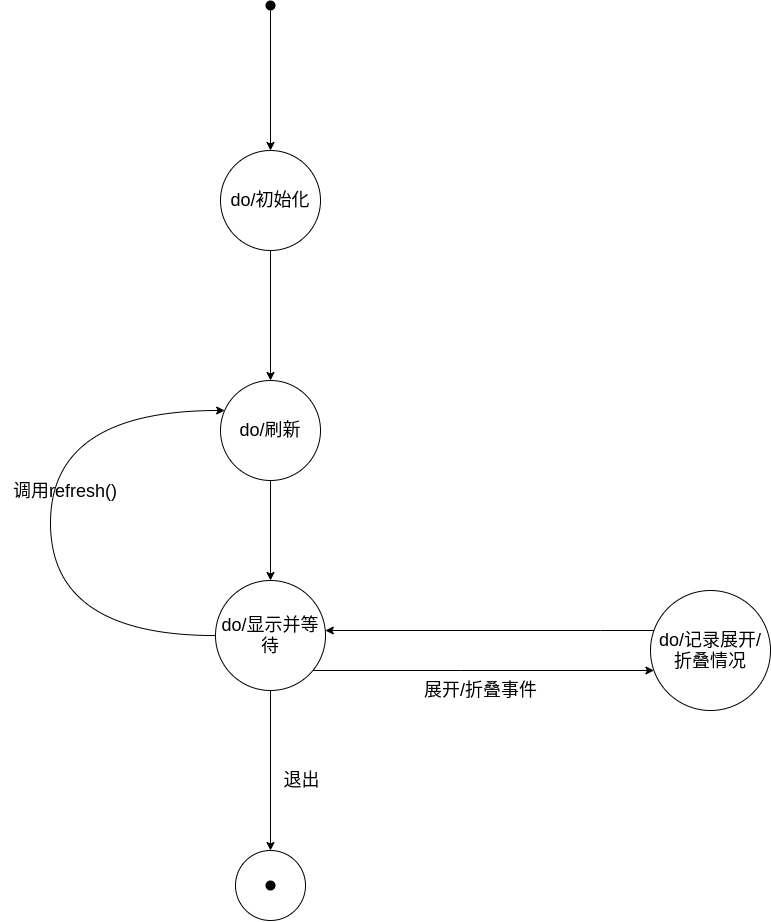
\includegraphics[scale=0.38]{../dia/user.png}
    \caption{\code{user}类状态图}
    \label{fig:userstat}
\end{figure}

用户页的功能是展示系统中所有用户和用户所创建的进程。这种结构通过\code{QTreeWidget}实现两层的树形布局,可以点击用户账户名称展开其创建的所有进程。

刷新时调用\code{QTreeWidget::clear()}清空所有内容,再重新填入新的用户和运行的进程。

当一个组件的下级组件被添加、删除时,这个组件会自动折叠。为了尽量保持更新前后视图一致,在\code{user}类中使用\code{std::vector<bool> expanded}记录各个用户组件的展开情况,刷新时访问\code{expanded}决定是否展开某个用户的进程:如果刷新前后用户数量不变,则认为用户没有发生变化,展开上次展开过的用户;若刷新后用户数量改变,则更新\code{expanded}的值为全\code{false},折叠所有用户组件。

\code{expanded}的更新通过slot \code{do\_expanded()}和\code{do\_collapsed()}实现,这两个函数使用\code{QTreeWid-\linebreak get::indexOfTopLevelItem()}获取被展开或折叠的用户组件序号,据此更改\code{expanded}中的元素。

\code{do\_expanded()}与\code{do\_collapsed()}代码如下:

{
    \ttfamily
    \lstinputlisting[breaklines=true,linerange={77-85},firstnumber=77]{../source/user.cc}
}

刷新时\code{user::refresh()}中根据\code{expanded}确定是否展开:

{
    \ttfamily
    \lstinputlisting[breaklines=true,linerange={70-73},firstnumber=70]{../source/user.cc}
}

\subsection{性能页的实现}
\label{subsec:perf}
状态图见图\myref{fig:perfstat}。

\begin{figure}[htb]
    \centering
    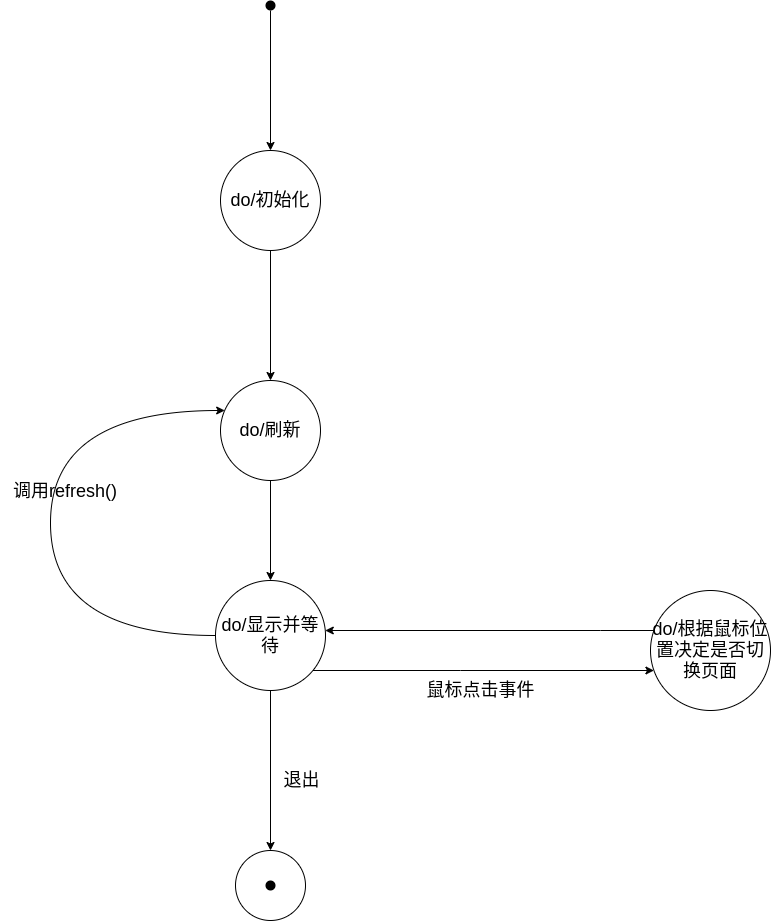
\includegraphics[scale=0.4]{../dia/performance.png}
    \caption{\code{performance}类状态图}
    \label{fig:perfstat}
\end{figure}

性能页由CPU页、内存页和两个缩略图组成。

CPU页和内存页的布局采用\code{QStackLayout},同一时刻两者只能有一个显示。

为了达到点击缩略图显示对应详细页面的效果,增加了鼠标点击事件发生时发射的signal \code{clicked}。将\code{clicked}与\code{mouseClicked()}关联,当\code{clicked}发射时\code{mouseClicked()}检查点击区域是否位于其中一个缩略图之内,若是,则使用\code{QStackLayout::setCurrentIndex()}设置此页面为当前页面:

{
    \ttfamily
    \lstinputlisting[breaklines=true,linerange={45-51},firstnumber=45]{../source/performance.cc}
}

性能页主要用于展示,交互功能只有以上一个。

\subsubsection{\code{load}类的实现}
状态图见图\myref{fig:loadstat}。

\begin{figure}[htb]
    \centering
    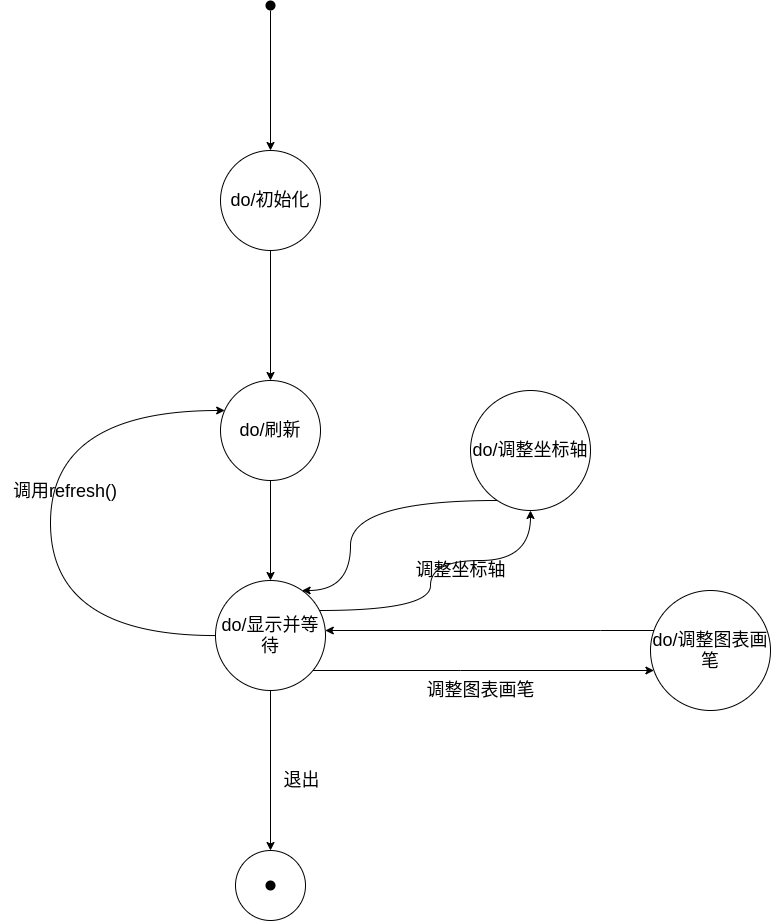
\includegraphics[scale=0.4]{../dia/load.png}
    \caption{\code{load}类状态图}
    \label{fig:loadstat}
\end{figure}

CPU页面,内存页面和缩略图都使用了\code{load}类以实现实时数据图表显示。

绘图功能使用Qt的Charts模块。这不属于Qt Core,为了使用Charts模块,需要在\ .pro文件中加入:

\begin{quote}
    \ttfamily
    QT += charts
\end{quote}

\code{load}类使用样条曲线作图。创建一个\code{QSplineSeries}类的实例,设置与其绑定的X轴与Y轴值域分别为$[-60s,0s]$和$[0,100]$。X轴的值域设置是为了显示$60s$内的数据变化情况,且最新的数据在最右侧,和Win10任务管理器一致。

更新时首先判断最旧的点横坐标值,即其创建的时刻是否距现在已超过$60s$。若是则删除这一点,否则直接添加新的一点。这样就达到了实时数据的刷新:

{
    \ttfamily
    \lstinputlisting[breaklines=true,linerange={60-68},firstnumber=60]{../source/load.cc}
}

\code{load}类还提供了\code{setSeriesPen()},\code{setXtick()}等函数供设置绘制风格。

\section{Taskmgr的部署}
把ico格式的图标放入项目文件夹,在 .pro项目文件中添加:
\begin{quote}
    \ttfamily
    RC\_ICONS = Taskmgr.ico
\end{quote}

Qt程序在运行时需要访问dll图形库,所以除了最终生成的exe文件外还需要把相关库放入合适的位置。

以Release模式生成可执行文件后将exe文件复制到目标文件夹,运行windeployqt Taskmgr.exe将需要的dll复制到目标文件夹下即可。只要拥有此文件夹,就可正常运行Taskmgr。

\section{功能与性能分析}
\label{sec:analyze}
% 没有规范的测试,由于时间和规模关系
% 界面与win10的对比……没实现的功能……与win10的不同之处的误差分析……(进程unkown……)
% 性能情况
% 性能瓶颈,内容耦合的合理性
\subsection{功能分析}
没有实现的功能已经在第\ref{sec:request} 节(p\pageref{sec:request})列出。

除了功能的不完全以外,已实现的功能中有一些问题:
\begin{itemize}
    \item CPU页面时钟频率始终是2.54GHz,但API调用应该没有错。可能是这个API比较古老,对处理器的支持不好
    \item 无法获取一些进程的信息,可能是因为需要比管理员更高的权限或者需要其他权限
    \item 界面不够美观
\end{itemize}

\subsection{与Win10任务管理器的对比}
在相近的时刻对Win10任务管理器和Taskmgr截图。见图\myref{fig:win10cpu},图\myref{fig:mgrcpu},图\myref{fig:win10mem},图\myref{fig:mgrmem}。

\begin{landscape}
\hspace{0pt}
\vfill

\begin{multicols}{2}
    
\begin{figure}[H]
    \centering
    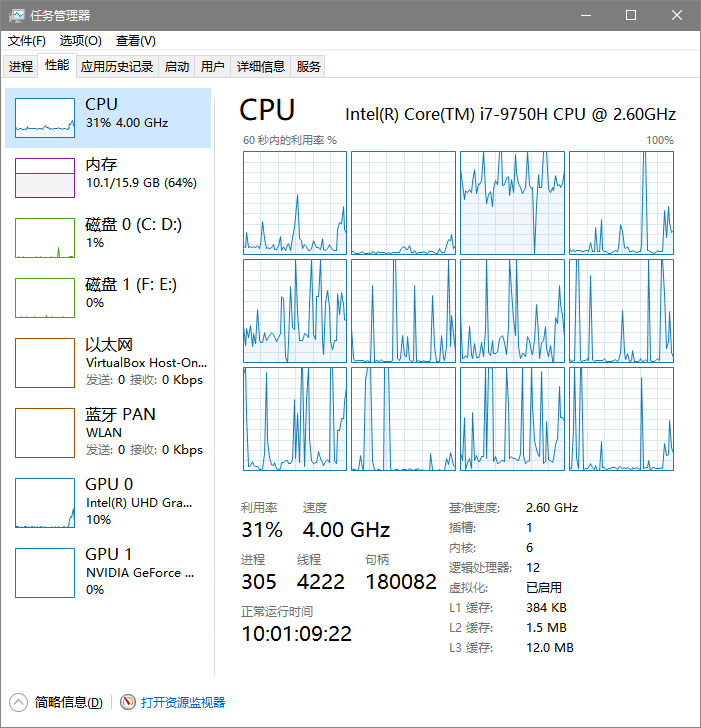
\includegraphics[scale=0.6]{../media/comparison/win10 perftab cpu.png}
    \caption{Win10任务管理器性能页-CPU}
    \label{fig:win10cpu}
\end{figure}

\columnbreak

\begin{figure}[H]
    \centering
    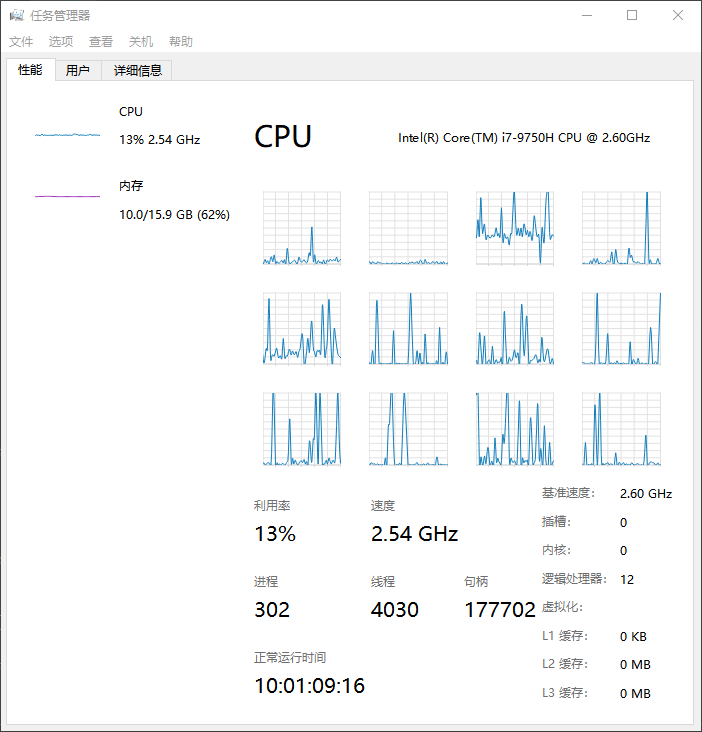
\includegraphics[scale=0.6]{../media/comparison/mgr perftab cpu.png}
    \caption{Taskmgr性能页-CPU}
    \label{fig:mgrcpu}
\end{figure}

\end{multicols}

\vfill
\hspace{0pt}
\end{landscape}

\begin{landscape}
\hspace{0pt}
\vfill

\begin{multicols}{2}

\begin{figure}[H]
    \centering
    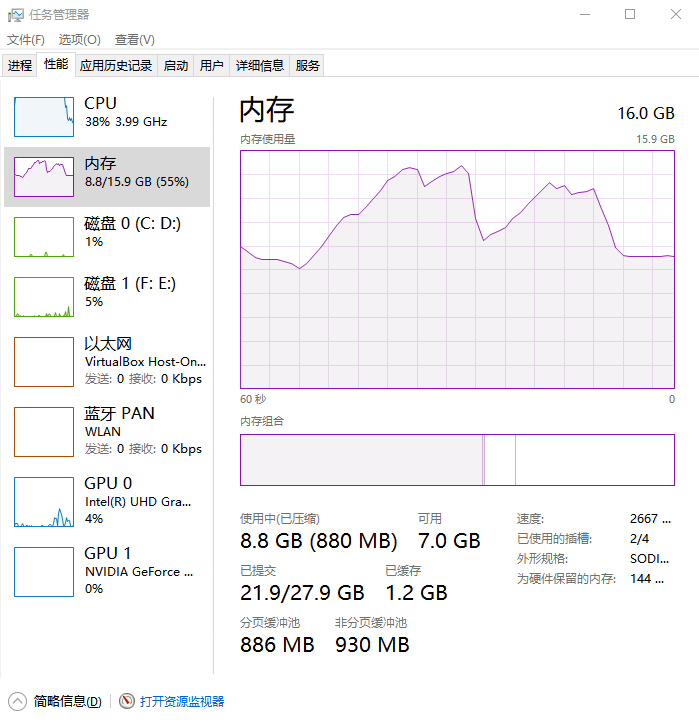
\includegraphics[scale=0.6]{../media/comparison/win10 perfTab mem.png}
    \caption{Win10任务管理器性能页-内存}
    \label{fig:win10mem}
\end{figure}

\columnbreak

\begin{figure}[H]
    \centering
    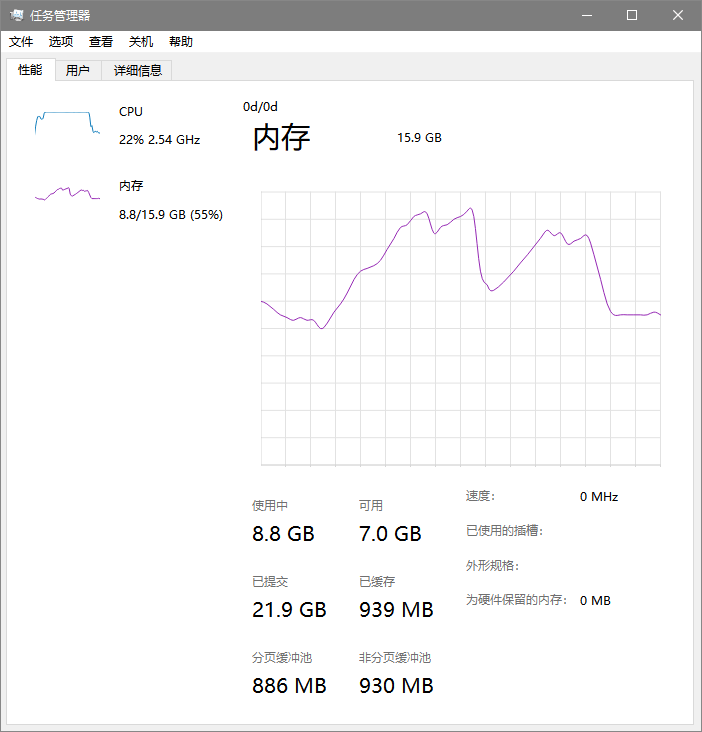
\includegraphics[scale=0.6]{../media/comparison/mgr perfTab mem.png}
    \caption{Taskmgr性能页-内存}
    \label{fig:mgrmem}
\end{figure}

\end{multicols}

\vfill
\hspace{0pt}
\end{landscape}

\subsection{性能分析}
主要从Taskmr消耗的CPU资源、内存资源和实际体验评价性能。最后通过qorbit注入采样分析程序的性能瓶颈。

这里通过Windows 10自带的任务管理器粗略地查看Taskmgr消耗的资源。不使用Taskmgr自身的原因是因为它是被测对象,而且功能也没有自带的任务管理器齐全。

刷新间隔为1s时,Taskmgr在性能页、用户页、详细信息页列表视图时消耗的CPU资源与内存分别为(1.8\%, 25.6MB), (1.6\%, 25.6MB, (2.0\%, 25.7MB)。(见图\myref{fig:perfanaly},图\myref{fig:useranaly},图\myref{fig:detailanaly})。这个资源占用是可以接受的。

\begin{figure}[htbp]
    \centering
    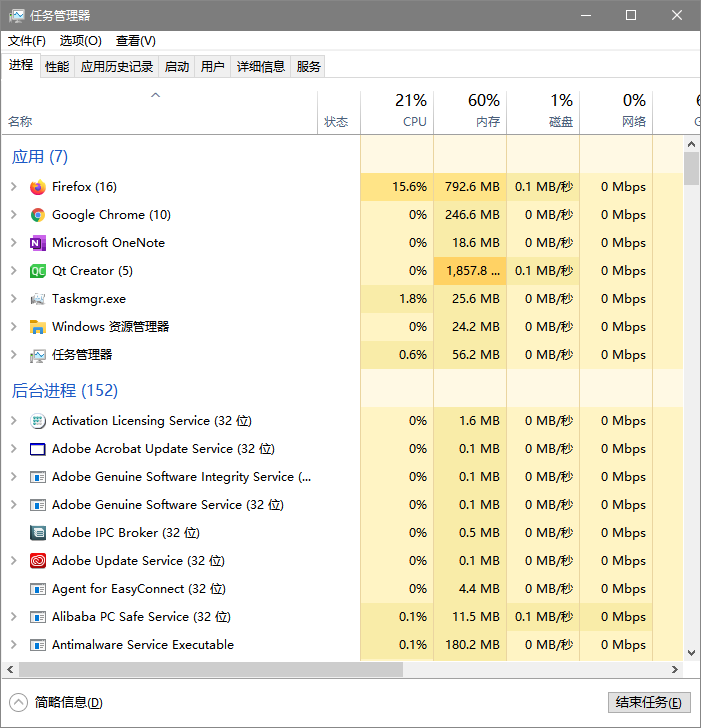
\includegraphics[scale=0.75,viewport=0 290 701 356,clip]{../media/performance analyze/load perftab.png}
    \caption{性能页时占用的资源}
    \label{fig:perfanaly}
\end{figure}

\begin{figure}[htbp]
    \centering
    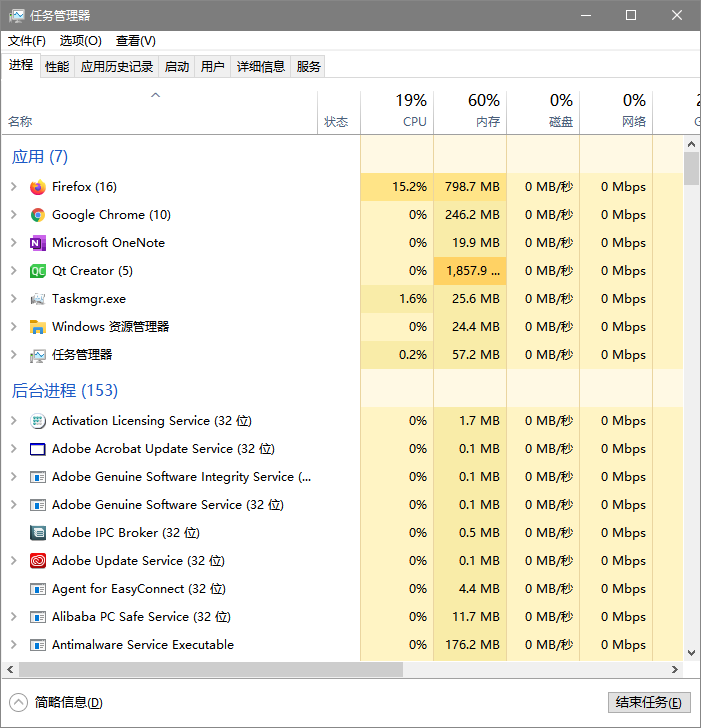
\includegraphics[scale=0.75,viewport=0 290 701 356,clip]{../media/performance analyze/load usertab.png}
    \caption{用户页时占用的资源}
    \label{fig:useranaly}
\end{figure}

\begin{figure}[htbp]
    \centering
    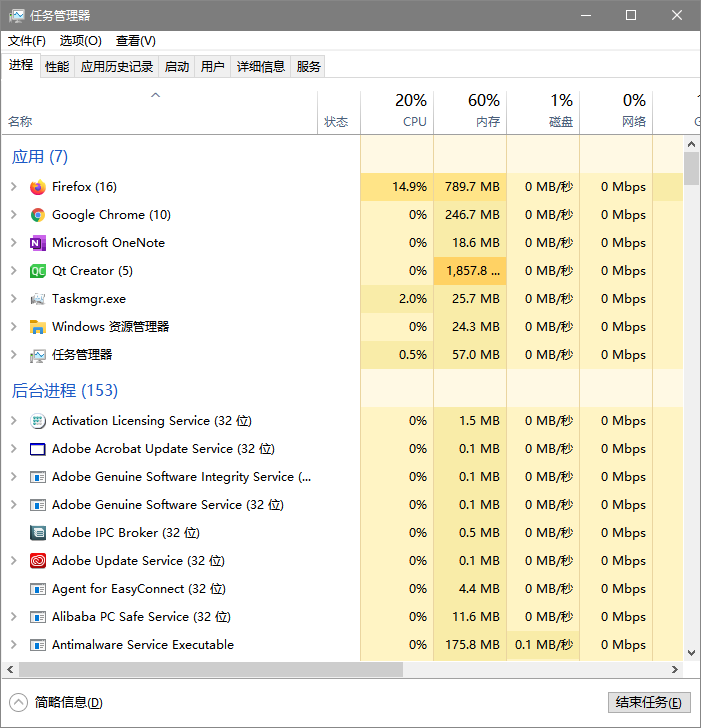
\includegraphics[scale=0.75,viewport=0 290 701 356,clip]{../media/performance analyze/load detailtab.png}
    \caption{详细信息页时占用的资源}
    \label{fig:detailanaly}
\end{figure}

从实际体验来看,即使刷新频率调为高,在各个Tab之间切换时没有卡顿,在详细信息页切换详细列表视图与图标视图时,以及鼠标滚动时也不会卡顿。

总的来说性能可以接受。

接下来通过注入采样分析性能瓶颈。

在1s的刷新间隔下,使用qorbit注入采样14.878s。结果见图\myref{fig:qorbit}。

\begin{figure}[H]
    \centering
    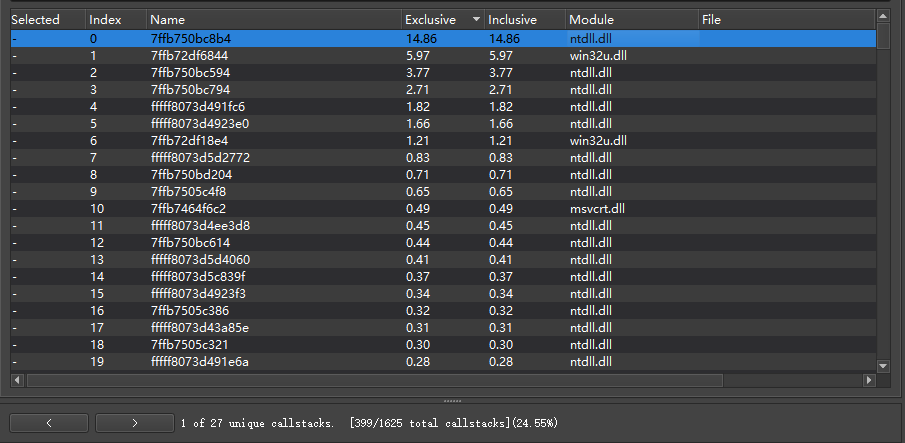
\includegraphics[scale=0.6]{../media/performance analyze/14.878s sampling result.png}
    \caption{注入采样结果(Exlusive time降序排序)}
    \label{fig:qorbit}
\end{figure}

占用exclusive时间最多的是ntdll.dll,比排序第二的win32u.dll高了近两倍。在ntdll.dll的调用栈中(见图\myref{fig:qorbit.1})可以看出在ntdll.dll调用的主要是读取虚拟内存、读取进程内存和读取进程的模块的函数。而在win32u.dll的调用栈中(见图\myref{fig:qorbit.2}),主要是用于绘图的函数与dll(\code{GetGlyphOutlineW}, Qt6Gui.dll等)。

\begin{figure}[H]
    \centering
    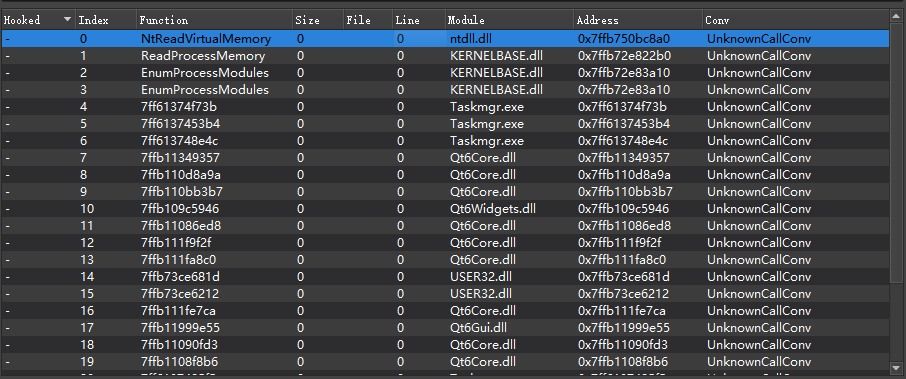
\includegraphics[scale=0.6]{../media/performance analyze/14.878s sampling result 1 callstuck.png}
    \caption{ntdll.dll的调用栈}
    \label{fig:qorbit.1}
\end{figure}

\begin{figure}[H]
    \centering
    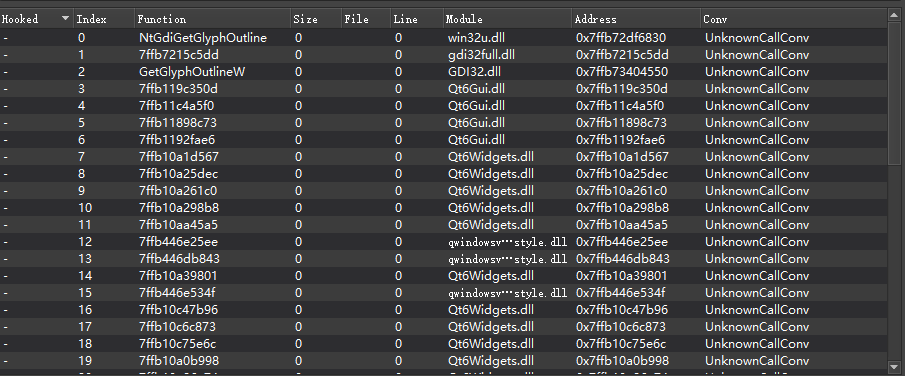
\includegraphics[scale=0.45]{../media/performance analyze/14.878s sampling result 2 callstuck.png}
    \caption{win32u.dll的调用栈}
    \label{fig:qorbit.2}
\end{figure}

由此可见,系统调用所花的时间是Taskmgr的性能瓶颈,对Taskmgr的优化应该在于降低win32 API调用频率。这也说明了此项目中出现内容耦合的合理性。

\end{document}
